
\chapter{Resultados}
\label{cha:resultados}

Aquí se mostrarán los resultados del proyecto \ldots

Como dijo \cite{lin2015microsoft} \ldots

\section{Introducción}
\label{sec:intro-resultados}

\section{Entorno experimental}
\label{sec:desarrollo-resultados}

\subsection{Bases de datos utilizadas}
\label{subsec:bases-datos}

\subsubsection{PETS2006 Dataset}

\begin{figure}[ht]
  \centering
  \begin{subfigure}[b]{0.4\textwidth}
    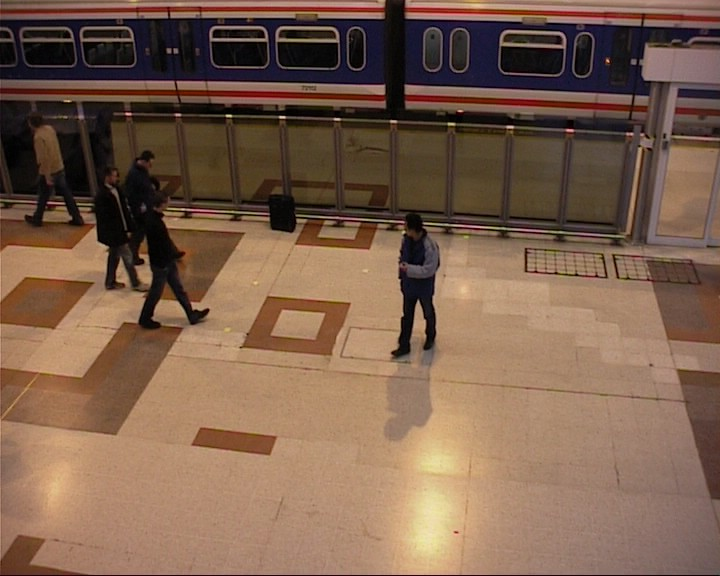
\includegraphics[width=\textwidth]{img/chapters/resultados/bases-datos/pets2006_1.jpeg}
    \caption{}
    \label{fig:pets2006_1}
  \end{subfigure}
  \qquad\qquad
  \begin{subfigure}[b]{0.4\textwidth}
    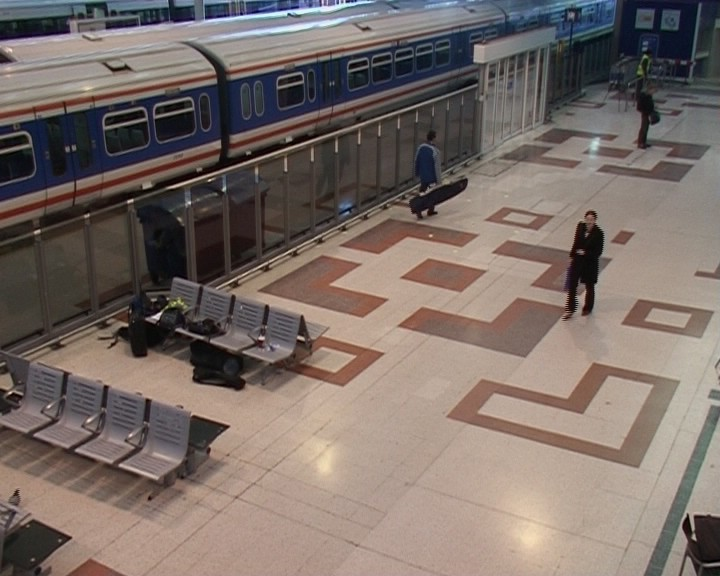
\includegraphics[width=\textwidth]{img/chapters/resultados/bases-datos/pets2006_2.jpeg}
    \caption{}
    \label{fig:pets2006_2}
  \end{subfigure}
  \caption{Imágenes extraídas del dataset PETS2006 \cite{pets2006-dataset}.
    (\protect\subref{fig:pets2006_1}) Frame donde una bolsa de equipaje se encuentra abandonada junto al andén.
    (\protect\subref{fig:pets2006_2}) Otro frame donde varias bolsas y maletas están abandonadas.}
  \label{fig:pets2006}
\end{figure}

\newpage

\subsubsection{PETS2007 Dataset}

\begin{figure}[ht]
  \centering
  \begin{subfigure}[b]{0.4\textwidth}
    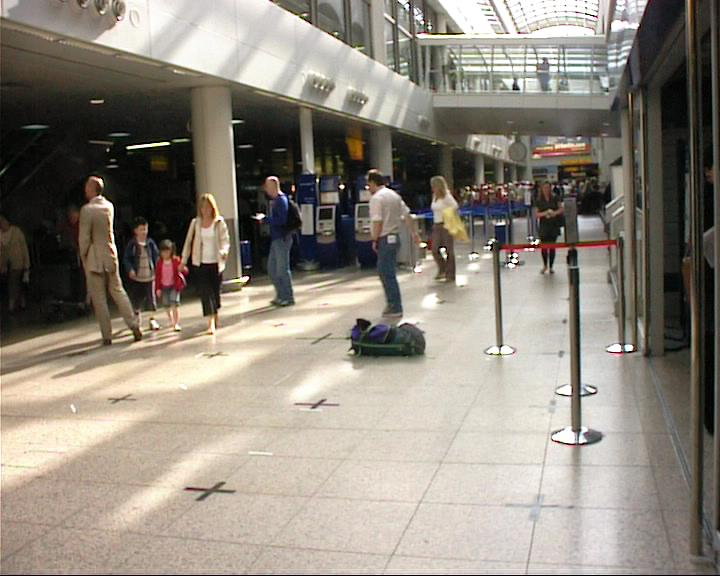
\includegraphics[width=\textwidth]{img/chapters/resultados/bases-datos/pets2007_1.jpeg}
    \caption{}
    \label{fig:pets2007_1}
  \end{subfigure}
  \qquad\qquad
  \begin{subfigure}[b]{0.4\textwidth}
    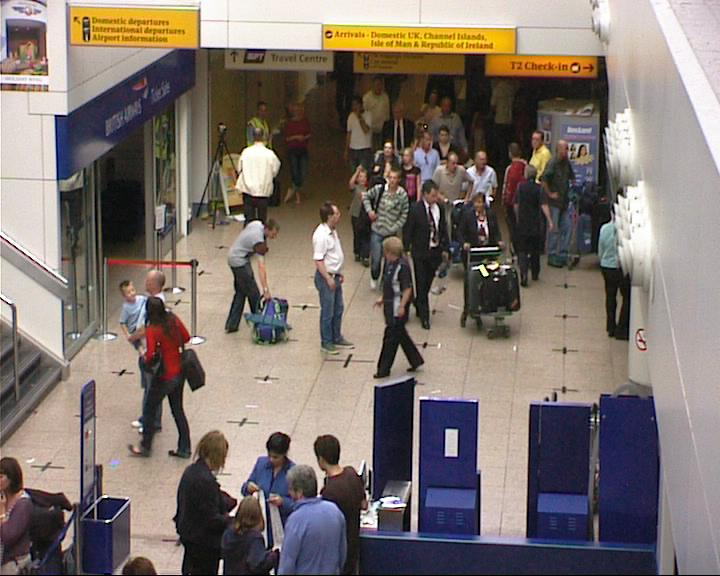
\includegraphics[width=\textwidth]{img/chapters/resultados/bases-datos/pets2007_2.jpeg}
    \caption{}
    \label{fig:pets2007_2}
  \end{subfigure}
  \caption{Imágenes extraídas del dataset PETS2007 \cite{pets2007-dataset}.
    (\protect\subref{fig:pets2007_1}) Frame donde un individuo deja su bolsa de equipaje sobre el suelo.
    (\protect\subref{fig:pets2007_2}) Otro frame en el cual una persona roba el equipaje el individuo.}
  \label{fig:pets2007}
\end{figure}

\subsubsection{AVSS AB 2007 Dataset}

\begin{figure}[ht]
  \centering
  \begin{subfigure}[b]{0.4\textwidth}
    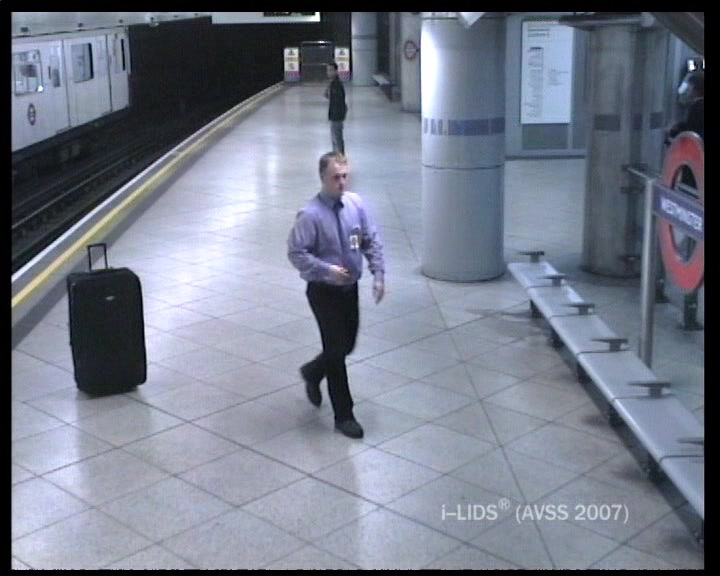
\includegraphics[width=\textwidth]{img/chapters/resultados/bases-datos/AVSSAB_1.jpg}
    \caption{}
    \label{fig:avssab2007_1}
  \end{subfigure}
  \qquad\qquad
  \begin{subfigure}[b]{0.4\textwidth}
    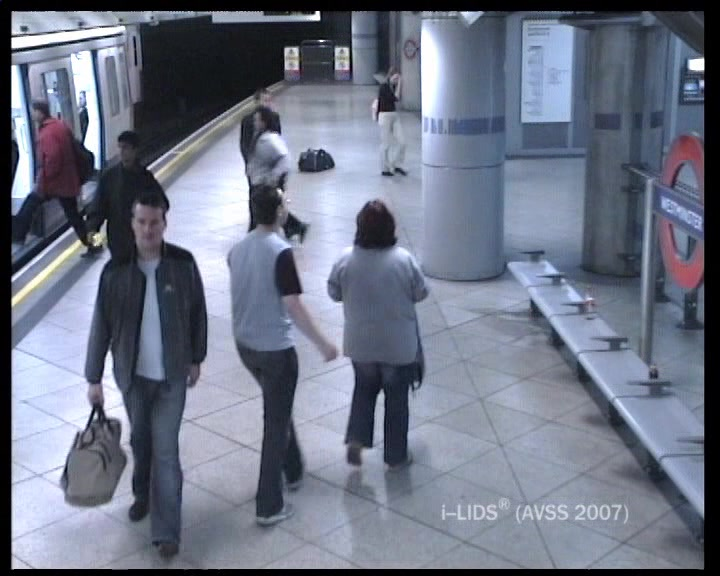
\includegraphics[width=\textwidth]{img/chapters/resultados/bases-datos/AVSSAB_2.jpg}
    \caption{}
    \label{fig:avssab2007_2}
  \end{subfigure}
  \caption{Imágenes extraídas del dataset AVSS AB 2007 \cite{AVSSAB2007-dataset}.
    (\protect\subref{fig:avssab2007_1}) Frame donde un individuo abandona su maleta en el andén.
    (\protect\subref{fig:avssab2007_2}) Otro frame donde una bolsa de equipaje está perdida en el andén durante todo el video.}
  \label{fig:avssab2007}
\end{figure}

\subsubsection{GBA Dataset}

\begin{figure}[ht!]
  \centering
  \begin{subfigure}[b]{0.45\textwidth}
    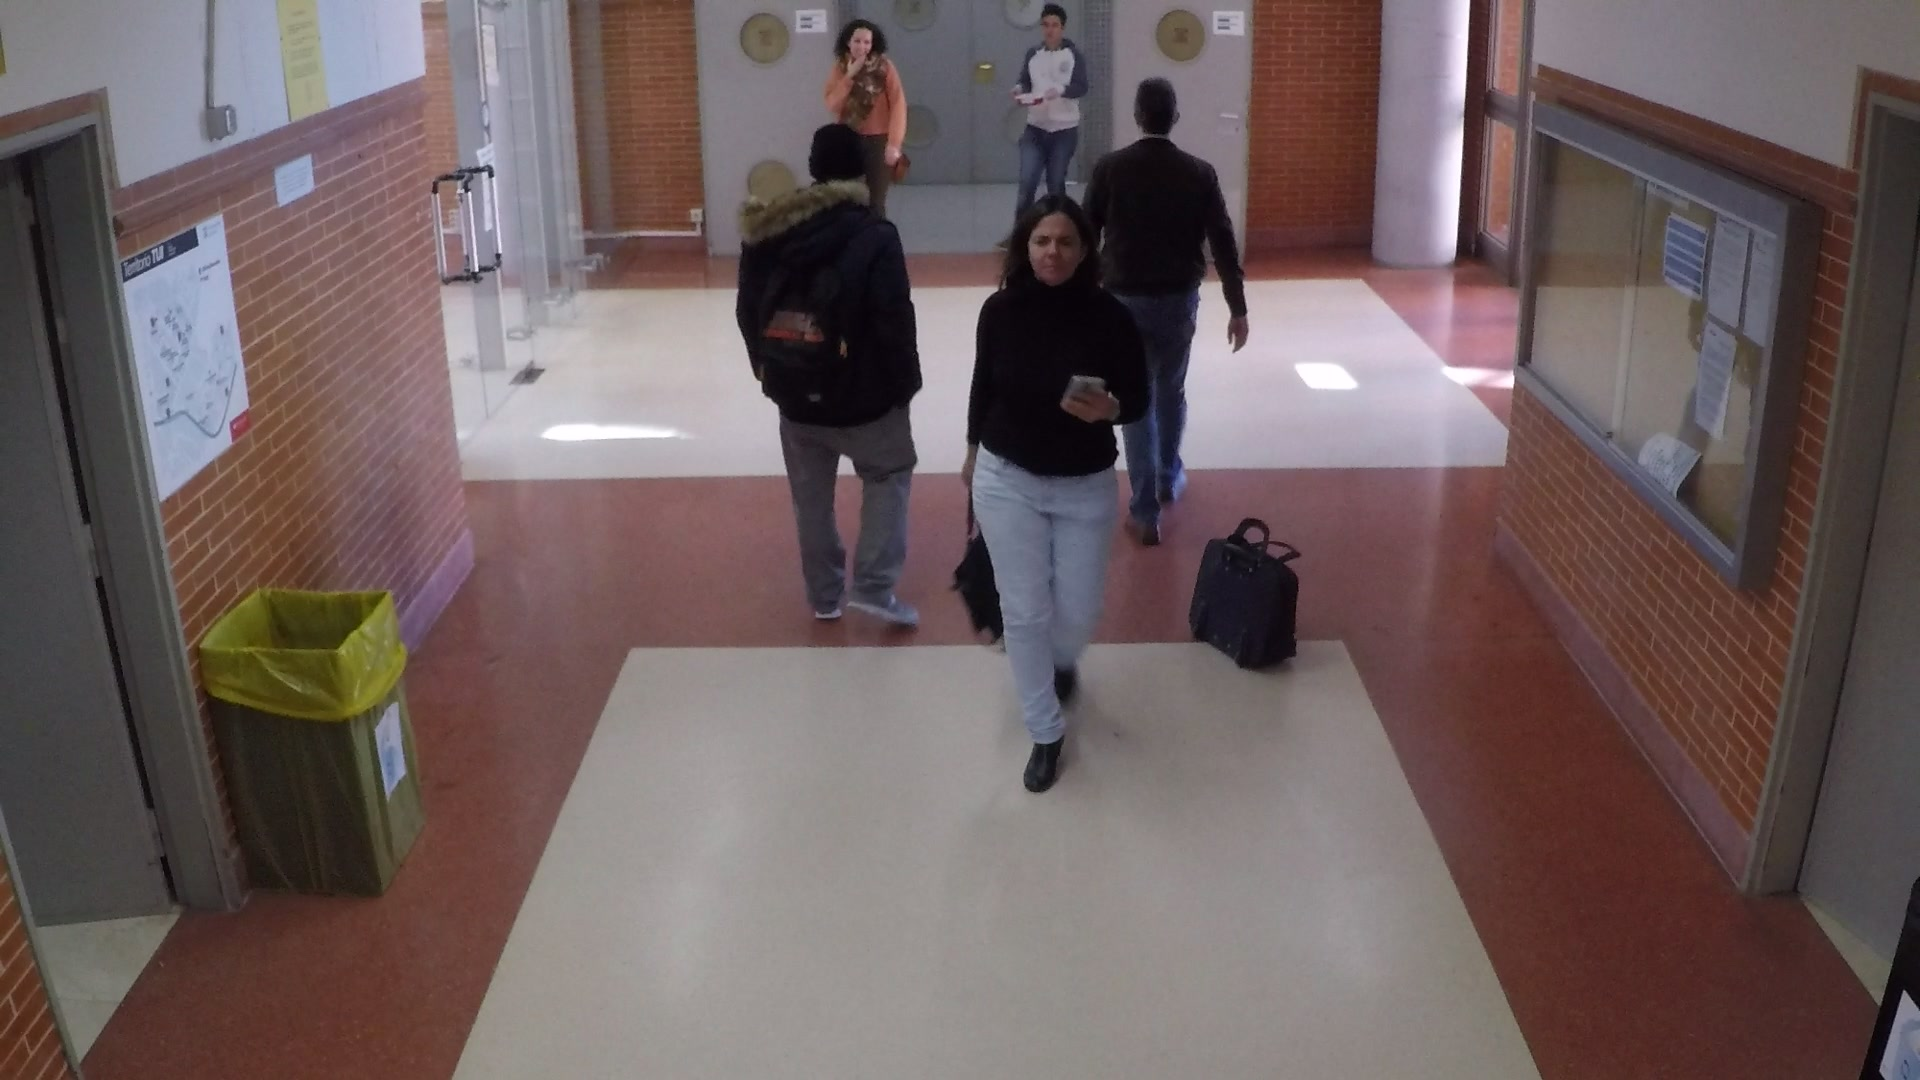
\includegraphics[width=\textwidth]{img/chapters/resultados/bases-datos/GBA_1.jpg}
    \caption{}
    \label{fig:GBA_1}
  \end{subfigure}
  \qquad\qquad
  \begin{subfigure}[b]{0.45\textwidth}
    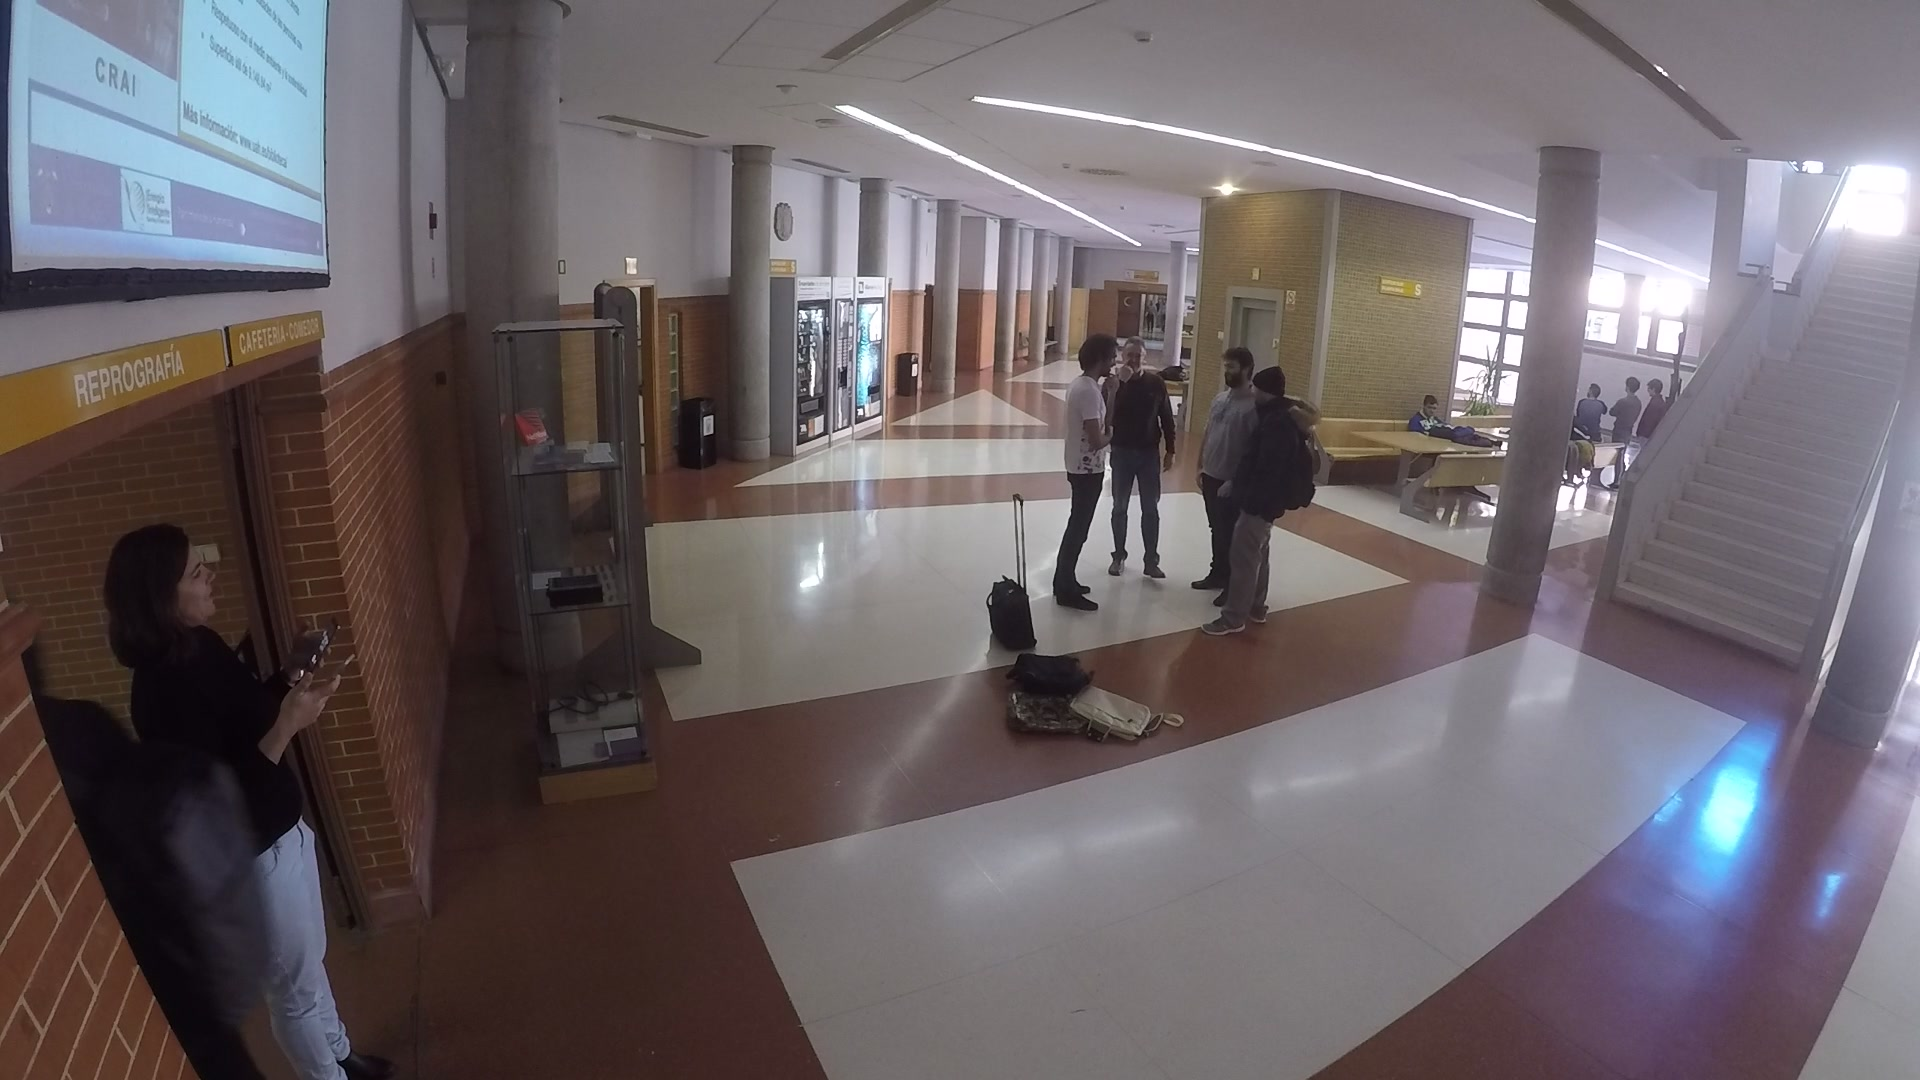
\includegraphics[width=\textwidth]{img/chapters/resultados/bases-datos/GBA_2.jpg}
    \caption{}
    \label{fig:GBA_2}
  \end{subfigure}
  \caption{Imágenes extraídas del dataset GBA \cite{gba-dataset}.
    (\protect\subref{fig:GBA_1}) Frame donde una bolsa de mano es abandonada en el pasillo.
    (\protect\subref{fig:GBA_2}) Otro frame donde varias bolsas y maletas están alejadas de sus propietarios.}
  \label{fig:GBA}
\end{figure}

\subsubsection{AVENUE Dataset}

\begin{figure}[ht]
  \centering
  \begin{subfigure}[b]{0.4\textwidth}
    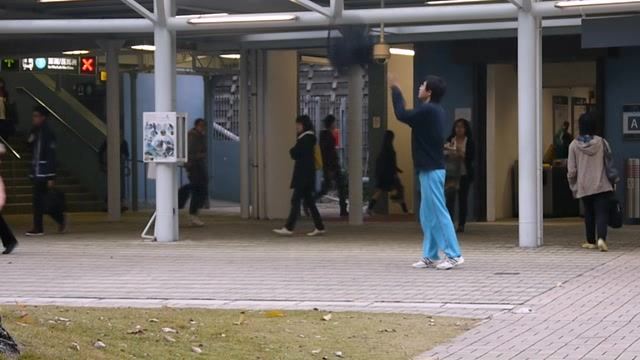
\includegraphics[width=\textwidth]{img/chapters/resultados/bases-datos/avenue_1.jpg}
    \caption{}
    \label{fig:avenue_1}
  \end{subfigure}
  \qquad\qquad
  \begin{subfigure}[b]{0.4\textwidth}
    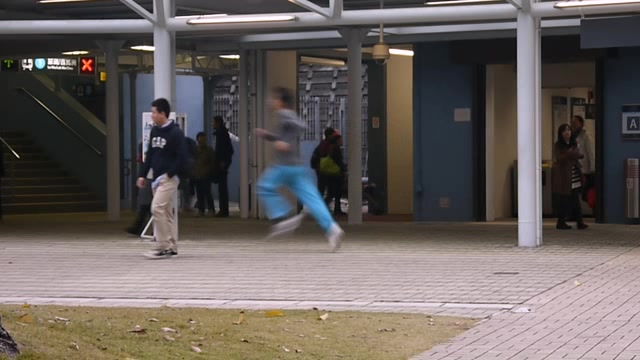
\includegraphics[width=\textwidth]{img/chapters/resultados/bases-datos/avenue_2.jpg}
    \caption{}
    \label{fig:avenue_2}
  \end{subfigure}
  \caption{Imágenes extraídas del dataset AVENUE \cite{avenue-dataset}.
    (\protect\subref{fig:avenue_1}) Frame donde un individuo lanza una mochila al aire.
    (\protect\subref{fig:avenue_2}) Otro frame donde un individuo corre de un lado a otro.}
  \label{fig:avenue}
\end{figure}

\subsubsection{ABODA Dataset}

\begin{figure}[ht]
  \centering
  \begin{subfigure}[b]{0.4\textwidth}
    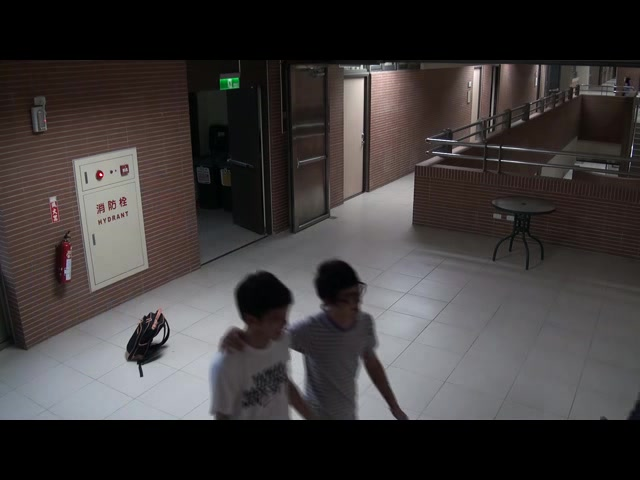
\includegraphics[width=\textwidth]{img/chapters/resultados/bases-datos/aboda_1.jpg}
    \caption{}
    \label{fig:aboda_1}
  \end{subfigure}
  \qquad\qquad
  \begin{subfigure}[b]{0.4\textwidth}
    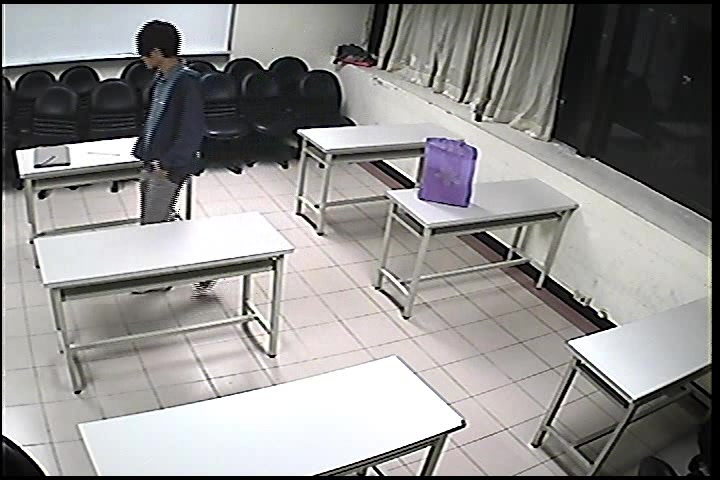
\includegraphics[width=\textwidth]{img/chapters/resultados/bases-datos/aboda_2.jpg}
    \caption{}
    \label{fig:aboda_2}
  \end{subfigure}
  \caption{Imágenes extraídas del dataset ABODA \cite{aboda-dataset}.
    (\protect\subref{fig:aboda_1}) Frame donde dos individuos se alejan de una mochila.
    (\protect\subref{fig:aboda_2}) Otro frame donde un individuo abandona una bolsa en la mesa.}
  \label{fig:aboda}
\end{figure}

\subsubsection{COCO Dataset}
\label{subsubsec:coco-dataset}

\textcolor{red}{La base de datos COCO es gran conjunto de datos que contiene más de 200 000 imágenes distribuidas en 80 clases de objetos que representan escenas del mundo real. Es una base de datos lo suficientemente grande para que una red bien entrenada con este conjunto de datos sea capaz de aprender características visuales de calidad para el reconocimiento y detección de objetos en imágenes.}

\begin{figure}[ht]
\centering
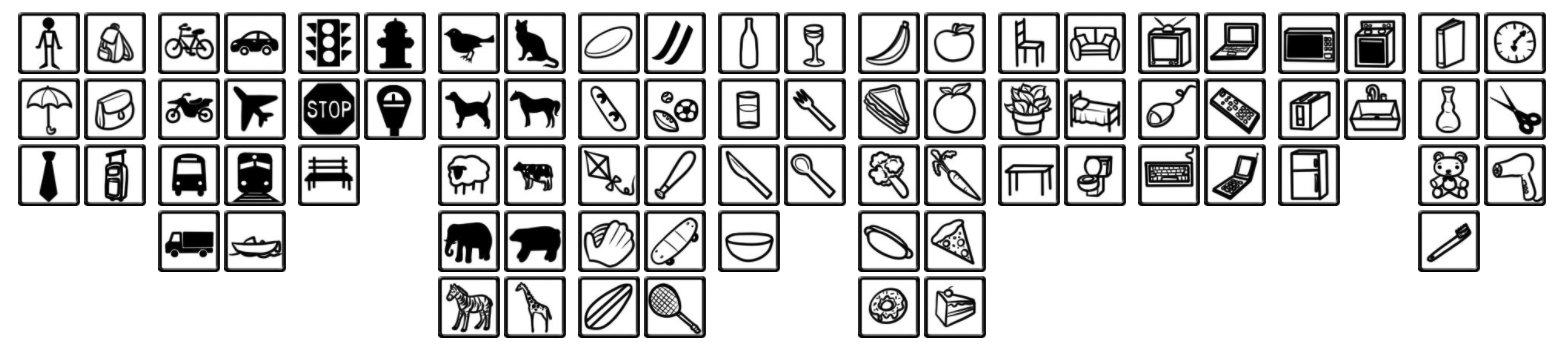
\includegraphics[width=0.9\textwidth]{img/chapters/resultados/bases-datos/cocodataset.png}
\caption{\label{fig:cocodataset}Categorías de objetos del dataset COCO}
\end{figure}

\subsection{Métricas de calidad}
\label{subsec:metricas-calidad}

\textcolor{red}{Ver TFM de Ana Ruipérez Gómez o Pedro López Miguel para ver como ha redactado las métricas} \pendiente{ojo a esto!!!}

En esta sección se va a exponer las distintas métricas \cite{padillaCITE2020} que han sido utilizadas para evaluar el conjunto de datos utilizado para el entrenamiento de la red neuronal.

\subsubsection{Intersección sobre la unión (IOU)}
\label{subsubsec:iou}

Intersection Over Union (IOU) es una medida basada en el índice Jaccard que evalúa la superposición entre dos cuadros delimitadores. Requiere un cuadro delimitador de verdad del terreno $B_{gt}$ y un cuadro delimitador previsto $B_{p}$. Aplicando el IOU podemos saber si una detección es válida (verdadero positivo) o no (falso positivo).

El IOU viene dado por el área de superposición entre el cuadro delimitador predicho y el cuadro delimitador de verdad del suelo dividido por el área de unión entre ellos:

\begin{equation}
\label{eq:iou}
\text{IOU}=\frac{\text{area}\left(B_{p} \cap B_{gt} \right)}{\text{area}\left(B_{p} \cup B_{gt} \right)}    
\end{equation}

La siguiente imagen ilustra el IOU entre un cuadro delimitador de verdad del terreno (en verde) y un cuadro delimitador detectado (en rojo).

\begin{figure}[ht]
\centering
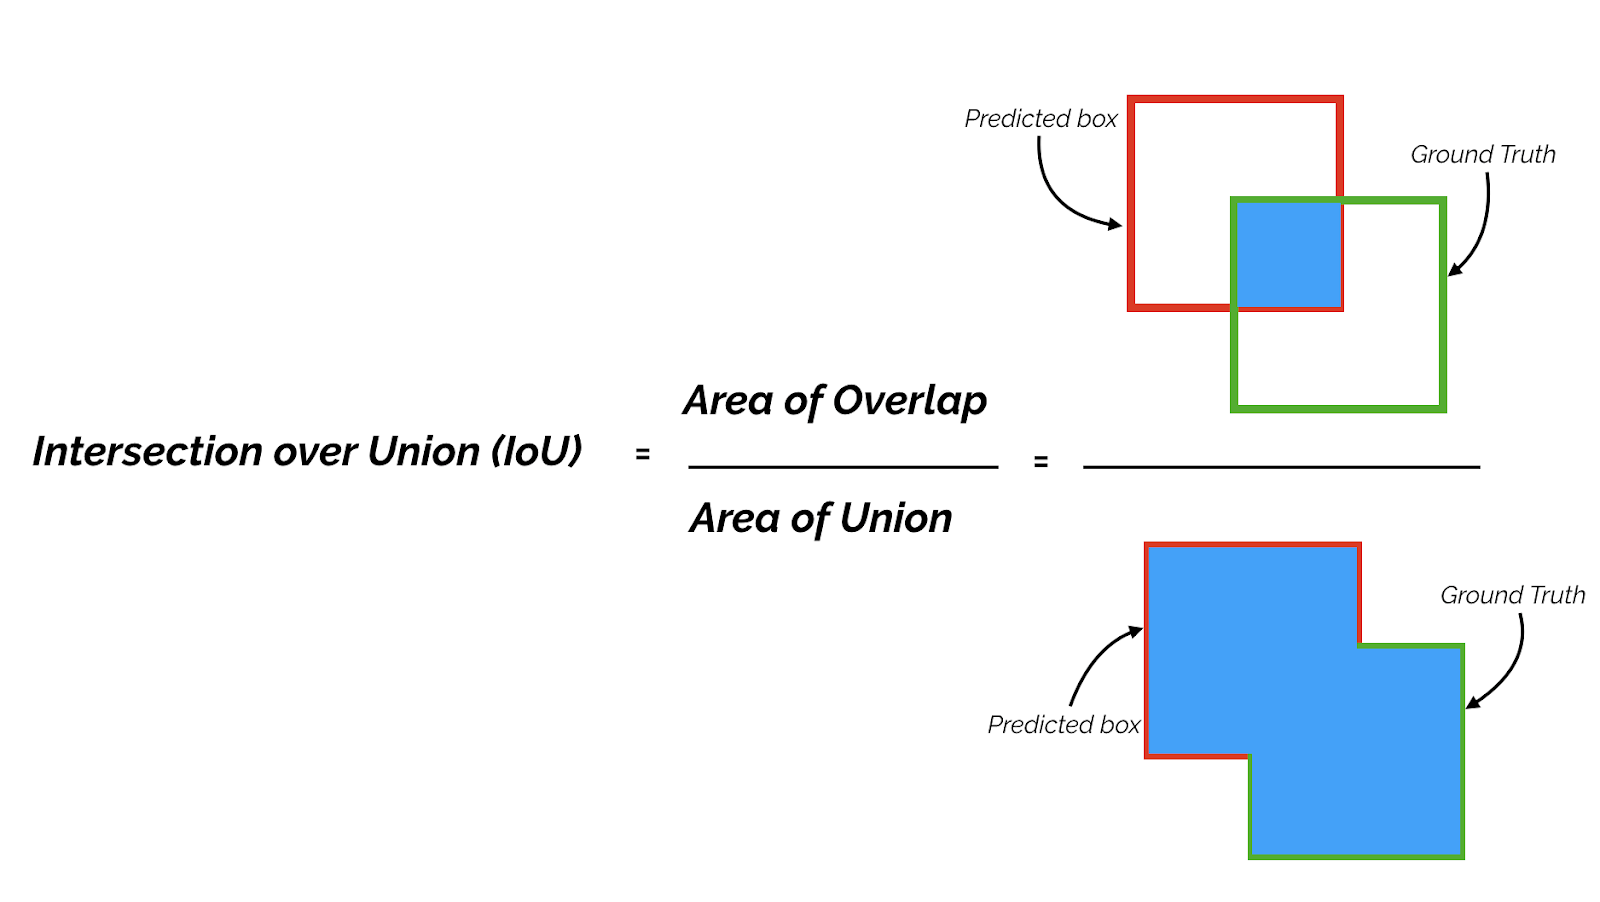
\includegraphics[width=0.45\textwidth]{img/chapters/resultados/metricas/iou.png}
\caption{\label{fig:iou}Área de superposición IOU entre los cuadros delimitadores}
\end{figure}

Algunos conceptos básicos que utilizan las métricas:

\begin{itemize}
    \item Verdadero positivo (TP): una detección correcta. Detección con IOU $\ge$ \textit{threshold}
    \item Falso positivo (FP): una detección incorrecta. Detección con IOU $<$ \textit{threshold}
    \item Falso negativo (FN): una verdad de tierra no detectada
    \item Verdadero negativo (TN): no se aplica. Representaría una detección errónea corregida. En la tarea de detección de objetos, hay muchos cuadros delimitadores posibles que no deben detectarse dentro de una imagen. Por lo tanto, TN serían todos los cuadros delimitadores posibles que no se detectaron correctamente (tantos cuadros posibles dentro de una imagen). Es por eso que las métricas no lo utilizan.
\end{itemize}

\textit{Threshold}: dependiendo de la métrica, generalmente se establece en 50\%, 75\% o 95\%.

\subsubsection{Precisión}
\label{subsubsec:precision}

La precisión es la capacidad de un modelo para identificar solo los objetos relevantes. Es el porcentaje de predicciones positivas correctas y viene dado por la siguiente expresión \ref{eq:precision}:

\begin{equation}
\label{eq:precision}
\text{Precision} = \frac{\text{TP}}{\text{TP}+\text{FP}}=\frac{\text{TP}}{\text{all detections}}
\end{equation}

\subsubsection{Recall}
\label{subsubsec:recall}

El \textit{Recall} es la capacidad de un modelo para encontrar todos los casos relevantes (todos los cuadros delimitadores de verdad del terreno). Es el porcentaje de verdadero positivo detectado entre todas las verdades fundamentales relevantes y viene dado por la siguiente expresión:


\begin{equation}
\label{eq:recall}
\text{Recall} = \frac{\text{TP}}{\text{TP}+\text{FN}}=\frac{\text{TP}}{\text{all ground truths}}
\end{equation}

\subsubsection{Precisión media}
\label{subsubsec:averageprecision}

La precisión media es el valor medio de 11 puntos en la curva P-R para cada posible umbral (cada probabilidad de detección) para la misma clase (Precisión-\textit{Recall}). En la ecuación \ref{eq:ap} se muestra el cálculo de la precisión media:

\begin{equation}
\label{eq:ap}
\text{AP}=\frac{1}{11} \sum_{r\in \left \{ 0, 0.1, ...,1 \right \}}\rho_{\text{interp}\left ( r \right )}
\end{equation}

con

$$\rho_{\text{interp}} = \max_{\tilde{r}:\tilde{r} \geq r} \rho\left ( \tilde{r} \right )$$

donde $\rho\left ( \tilde{r} \right )$ es la precisión medida en el \textit{Recall} $\tilde{r}$

Por otro lado, el mAP es la media de los AP de todas las categorías de objetos. el mAP se representa mediante la siguiente ecuación:

\begin{equation}
\label{eq:map}
\text{mAP} = \frac{1}{N} \sum_{i=1}^{N} \text{AP}_{1}
\end{equation}

\subsection{Estrategia y metodología de experimentación}
\label{subsec:estrategia-metodologia}

\newpage

\subsubsection{Entrenamiento con Open Image Dataset v4}
\label{subsubsec:train-openimagesv4}

\textcolor{red}{Aquí explicar como he entrado una red neuronal con otro dataset a partir del repositorio \cite{OIDv4_ToolKit}}

\newpage

\subsubsection{Métricas de calidad en Open Image Dataset v4}
\label{subsubsec:metricas-calidad-openimagesv4}

Tras entrenar YOLOv4 con el conjunto de datos personalizado que se ha explicado en el apartado anterior \ref{subsubsec:train-openimagesv4} se va a evaluar las métricas de calidad. Gracias al framework Darknet \cite{darknet13} es fácil poder evaluar las métricas aplicando el siguiente comando en el terminal:

\vspace{0.5cm}
\begin{lstlisting}[language=iPython,caption=Evaluación métricas de calidad del conjunto de datos utilizado para el entrenamiento de la red neuronal de detección de objetos,captionpos=b,label={lst:darknet-map}]
# Evaluacion de metricas de interes
./darknet detector map ./cfg/coco.data ./cfg/yolov4.cfg ./yolov4.weights
\end{lstlisting}

En la tabla \ref{tab:metricas-test1_1} y \ref{tab:metricas-test1_2} se reflejan las métricas más relevantes cada 1000 iteraciones del entrenamiento de la red neuronal.


\begin{table}[ht]
\centering
\caption{Métricas de calidad en test 1}
\label{tab:metricas-test1_1}
\begin{tabular}{|c|c|c|c|c|c|c|}
\hline
\rowcolor[HTML]{EFEFEF} 
\textbf{Iterations} & \textbf{\begin{tabular}[c]{@{}c@{}}AP person\\ (\%)\end{tabular}} & \textbf{\begin{tabular}[c]{@{}c@{}}AP bags\\ (\%)\end{tabular}} & \textbf{TP person} & \textbf{TP bags} & \textbf{FP person} & \textbf{FP bags} \\ \hline
1.000               & 28,55                                                             & 59,98                                                           & 2.287              & 411              & 6.170              & 372              \\ \hline
2.000               & 40,56                                                             & 82,92                                                           & 2.354              & 469              & 3.523              & 293              \\ \hline
3.000               & 37,32                                                             & 81,65                                                           & 2.383              & 457              & 3.854              & 285              \\ \hline
4.000               & 36,52                                                             & 80,37                                                           & 2.231              & 481              & 3.409              & 487              \\ \hline
5.000               & 38,89                                                             & 80,25                                                           & 2.430              & 460              & 3.946              & 324              \\ \hline
6.000               & 37,54                                                             & 80,02                                                           & 2.331              & 471              & 3.752              & 419              \\ \hline
\end{tabular}
\end{table}

\begin{table}[ht]
\centering
\caption{Métricas de calidad en test 1}
\label{tab:metricas-test1_2}
\begin{tabular}{|c|c|c|c|c|c|c|c|}
\hline
\rowcolor[HTML]{EFEFEF} 
\textbf{Iterations} & \textbf{TP} & \textbf{FP} & \textbf{FN} & \textbf{\begin{tabular}[c]{@{}c@{}}Precision\\ (\%)\end{tabular}} & \textbf{\begin{tabular}[c]{@{}c@{}}Recall\\ (\%)\end{tabular}} & \textbf{\begin{tabular}[c]{@{}c@{}}average IoU\\ (\%)\end{tabular}} & \textbf{\begin{tabular}[c]{@{}c@{}}mAP @ 0.5\\ (\%)\end{tabular}} \\ \hline
1.000               & 2.698       & 6.542       & 2.037       & 29,20                                                             & 56,98                                                          & 20,72                                                               & 44,27                                                             \\ \hline
2.000               & 2.823       & 3.816       & 1.912       & 42,52                                                             & 59,62                                                          & 33,26                                                               & 61,74                                                             \\ \hline
3.000               & 2.840       & 4.139       & 1.895       & 40,69                                                             & 59,98                                                          & 31,99                                                               & 59,48                                                             \\ \hline
4.000               & 2.712       & 3.896       & 2.023       & 41,04                                                             & 57,28                                                          & 32,06                                                               & 58,44                                                             \\ \hline
5.000               & 2.890       & 4.270       & 1.845       & 40,36                                                             & 61,03                                                          & 32,13                                                               & 59,57                                                             \\ \hline
6.000               & 2.802       & 4.171       & 1.923       & 40,18                                                             & 61,03                                                          & 31,49                                                               & 58,17                                                             \\ \hline
\end{tabular}
\end{table}

\textcolor{red}{Aquí explicar porque en función de las métricas obtenidas no es un buen modelo y se debe de reentrenar la red}

\newpage

\begin{table}[ht]
\centering
\caption{Métricas de calidad test 2}
\label{tab:metricas-test2_1}
\begin{tabular}{|c|c|c|c|c|c|c|}
\hline
\rowcolor[HTML]{EFEFEF} 
\textbf{Iterations} & \textbf{\begin{tabular}[c]{@{}c@{}}AP person\\ (\%)\end{tabular}} & \textbf{\begin{tabular}[c]{@{}c@{}}AP bags\\ (\%)\end{tabular}} & \textbf{TP person} & \textbf{TP bags} & \textbf{FP person} & \textbf{FP bags} \\ \hline
1.000               & 30,81                                                             & 21,61                                                          & 5.216              & 231             & 9.220              & 579             \\ \hline
2.000               & 38,38                                                             & 53,59                                                          & 6.542              & 362             & 11.789             & 354             \\ \hline
3.000               & 33,51                                                             & 68,56                                                          & 7.232              & 419             & 18.887             & 411             \\ \hline
4.000               & 41,31                                                             & 77,12                                                          & 7.105              & 427             & 11.397             & 222             \\ \hline
5.000               & 38,86                                                             & 75,78                                                          & 6.586              & 444             & 11.735             & 398             \\ \hline
6.000               & 36,29                                                             & 66,49                                                          & 6.556              & 426             & 12.506             & 537             \\ \hline
7.000               & 39,94                                                             & 67,78                                                          & 6.246              & 418             & 9.744              & 523             \\ \hline
8.000               & 31,69                                                             & 69,07                                                          & 6.082              & 417             & 13.353             & 422             \\ \hline
9.000               & 43,34                                                             & 78,37                                                          & 6.773              & 451             & 9.846              & 373             \\ \hline
10.000              & 43,40                                                             & 78,53                                                          & 6.174              & 426             & 7.149              & 217             \\ \hline
11.000              & 38,81                                                             & 76,60                                                          & 7.166              & 446             & 12.162             & 387             \\ \hline
12.000              & 41,72                                                             & 78,10                                                          & 6.926              & 444             & 10.387             & 289             \\ \hline
13.000              & 39,48                                                             & 74,67                                                          & 6.575              & 406             & 9.850              & 238             \\ \hline
14.000              & 41,85                                                             & 73,69                                                          & 6.844              & 432             & 10.092             & 385             \\ \hline
15.000              & 40,19                                                             & 75,37                                                          & 6.915              & 423             & 11.426             & 252             \\ \hline
16.000              & 41,26                                                             & 75,17                                                          & 6.661              & 423             & 9.330              & 219             \\ \hline
17.000              & 42,13                                                             & 78,77                                                          & 6.991              & 433             & 9.924              & 242             \\ \hline
18.000              & 40,97                                                             & 75,45                                                          & 6.871              & 432             & 10.243             & 300             \\ \hline
19.000              & 39,01                                                             & 73,23                                                          & 6.822              & 428             & 10.791             & 333             \\ \hline
20.000              & 41,37                                                             & 78,38                                                          & 7.011              & 432             & 10.103             & 232             \\ \hline
\end{tabular}
\end{table}
\aviso{Estas dos tablas tienen que ir solas en una página para que no se raye el documento poniendo las tablas donde le da la gana}
\begin{table}[ht!]
\centering
\caption{Métricas de calidad test 2}
\label{tab:metricas-test2_2}
\begin{tabular}{|c|c|c|c|c|c|c|c|}
\hline
\rowcolor[HTML]{EFEFEF} 
\textbf{Iterations} & \textbf{TP} & \textbf{FP} & \textbf{FN} & \textbf{\begin{tabular}[c]{@{}c@{}}Precision\\ (\%)\end{tabular}} & \textbf{\begin{tabular}[c]{@{}c@{}}Recall\\ (\%)\end{tabular}} & \textbf{\begin{tabular}[c]{@{}c@{}}average\\ IoU (\%)\end{tabular}} & \textbf{\begin{tabular}[c]{@{}c@{}}mAP\\ @ 0.5 (\%)\end{tabular}} \\ \hline
1.000               & 5.447       & 9.799       & 6.379       & 35,73                                                             & 46,06                                                          & 25,72                                                               & 26,21                                                             \\ \hline
2.000               & 6.904       & 12.143      & 4.922       & 36,25                                                             & 58,38                                                          & 27,30                                                               & 45,98                                                             \\ \hline
3.000               & 7.651       & 19.298      & 4.175       & 28,39                                                             & 64,70                                                          & 21,66                                                               & 51,04                                                             \\ \hline
4.000               & 7.532       & 11.619      & 4.294       & 39,33                                                             & 63,69                                                          & 30,90                                                               & 59,22                                                             \\ \hline
5.000               & 7.030       & 12.133      & 4.796       & 36,69                                                             & 59,45                                                          & 28,28                                                               & 57,32                                                             \\ \hline
6.000               & 6.982       & 13.043      & 4.844       & 34,87                                                             & 59,04                                                          & 27,23                                                               & 51,39                                                             \\ \hline
7.000               & 6.664       & 10.267      & 5.162       & 39,36                                                             & 56,35                                                          & 30,96                                                               & 53,86                                                             \\ \hline
8.000               & 6.499       & 13.775      & 5.327       & 32,06                                                             & 54,96                                                          & 24,96                                                               & 50,38                                                             \\ \hline
9.000               & 7.224       & 10.219      & 4.602       & 41,41                                                             & 61,09                                                          & 32,95                                                               & 60,85                                                             \\ \hline
10.000              & 6.600       & 7.366       & 5.226       & 47,26                                                             & 55,81                                                          & 37,83                                                               & 60,97                                                             \\ \hline
11.000              & 7.612       & 12.549      & 4.214       & 37,76                                                             & 64,37                                                          & 30,20                                                               & 57,70                                                             \\ \hline
12.000              & 7.370       & 10.676      & 4.456       & 40,84                                                             & 62,32                                                          & 32,34                                                               & 59,91                                                             \\ \hline
13.000              & 6.981       & 10.088      & 4.845       & 40,90                                                             & 59,03                                                          & 32,83                                                               & 57,07                                                             \\ \hline
14.000              & 7.276       & 10.477      & 4.550       & 40,98                                                             & 61,53                                                          & 32,61                                                               & 57,77                                                             \\ \hline
15.000              & 7.338       & 11.678      & 4.488       & 38,59                                                             & 62,05                                                          & 30,53                                                               & 57,78                                                             \\ \hline
16.000              & 7.084       & 9.549       & 4.742       & 42,59                                                             & 59,90                                                          & 33,87                                                               & 58,22                                                             \\ \hline
17.000              & 7.424       & 10.166      & 4.402       & 42,21                                                             & 62,78                                                          & 34,53                                                               & 60,45                                                             \\ \hline
18.000              & 7.303       & 10.543      & 4.523       & 40,92                                                             & 61,75                                                          & 33,11                                                               & 58,21                                                             \\ \hline
19.000              & 7.250       & 11.124      & 4.576       & 39,46                                                             & 61,31                                                          & 31,90                                                               & 56,12                                                             \\ \hline
20.000              & 7.443       & 10.335      & 4.383       & 41,87                                                             & 62,94                                                          & 34,35                                                               & 59,93                                                             \\ \hline
\end{tabular}
\end{table}

\newpage

\subsubsection{Métricas de calidad en COCO dataset}
\label{subsubsec:metricas-calidad-coco}

\begin{table}[ht]
\centering
\caption{Comparativa métricas de calidad entre los dos test en Open Images v6 y COCO}
\label{tab:comparativa-metricas}
\begin{tabular}{|c|c|c|c|c|c|c|c|}
\hline
\rowcolor[HTML]{EFEFEF} 
\textbf{Dataset}                                                & \textbf{TP} & \textbf{FP} & \textbf{FN} & \textbf{\begin{tabular}[c]{@{}c@{}}Precision\\ (\%)\end{tabular}} & \textbf{\begin{tabular}[c]{@{}c@{}}Recall\\ (\%)\end{tabular}} & \textbf{\begin{tabular}[c]{@{}c@{}}average IoU\\ (\%)\end{tabular}} & \textbf{\begin{tabular}[c]{@{}c@{}}mAP @ 0.5\\ (\%)\end{tabular}} \\ \hline
COCO 2017                                                       & 22.730      & 10.889      & 13.027      & 67,61                                                             & 63,57                                                          & 56,04                                                               & 64,16                                                             \\ \hline
\begin{tabular}[c]{@{}c@{}}Open Images v4\\ test 1\end{tabular} & 2.823       & 3.816       & 1.912       & 42,52                                                             & 59,62                                                          & 33,26                                                               & 61,74                                                             \\ \hline
\begin{tabular}[c]{@{}c@{}}Open Images v4\\ test 2\end{tabular} & 6.600       & 7.366       & 5.226       & 47,26                                                             & 55,81                                                          & 37,83                                                               & 60,97                                                             \\ \hline
\end{tabular}
\end{table}

\begin{table}[ht]
\centering
\caption{Métricas de calidad en COCO}
\label{tab:metricas-coco}
\begin{tabular}{|c|c|c|c|}
\hline
\rowcolor[HTML]{EFEFEF} 
\textbf{Class} & \textbf{AP (\%)} & \textbf{TP} & \textbf{FP} \\ \hline
person         & 79,21            & 8.078       & 2.836       \\ \hline
backpack       & 44,23            & 172         & 148         \\ \hline
handbag        & 29,59            & 157         & 206         \\ \hline
suitcase       & 71,03            & 207         & 96         \\ \hline
\end{tabular}
\end{table}


\section{Resultados experimentales}
\label{sec:resultados-experimentales}

Una vez elegido COCO dataset como conjunto de datos de referencia para usar con YOLOv4, se va a ver los resultados obtenidos en distintos algoritmos.

\subsection{Resultados en detección de objetos con YOLOv4}
\label{subsec:resultados-yolov4-tf}

\textcolor{red}{Poner imágenes de las detecciones en los datasets empleados y explicar con detalle como influye distintos elementos como la distancia, iluminación, color, etc... en la detección de objetos}.

\subsection{Resultados en tracking con DeepSORT}
\label{subsec:resultados-deepsort}

\textcolor{red}{Poner imágenes de las detecciones en los datasets empleados y explicar con detalle los problemas con los que nos podemos encontrar a la hora de hacer un seguimiento o \textit{tracking} de objetos y personas, se pierde el rastreo y se vuelve a asociar una nueva ID a ese individuo, también explicar que debido al \textit{threshold} que pongamos se pueden perder objetos, pero tampoco es conveniente bajarlo a más de X porque entonces se confunden objetos o se trackean varias veces}.

\subsection{Resultados en algoritmo de detección de objetos abandonados}
\label{subsec:resultados-abandon-algorithm}

\textcolor{red}{Poner imágenes de detecciones de objetos abandonados y explicar de manera visual como es posible que hayan problemas cuando se pierde el \textit{tracking} de un objeto o persona y se tiene que reasignar como nuevo ID y posteriormente tener que volver a hacer una asociación de persona-objeto y evaluar si se abandona o no dicho objeto}.

\textcolor{red}{Aquí meter un subsubapartado con métricas relevantes en la detección de objetos abandonados}.

\section{Conclusiones}
\label{sec:conclu-resultados}